%!TEX TS-program = pdflatex
\documentclass[12pt]{article}  % larger font to compensate for long lines with fullpage
\usepackage{graphicx}
\usepackage{ifpdf,ifxetex}

\ifxetex
% \usepackage{fontspec}
\else % inputenc is incompatible with xetex (which always takes UTF-8 as input)
\usepackage[utf8]{inputenc}
\fi
\usepackage{ifthen}
\usepackage[pdfborder={0 0 0}]{hyperref} % use hyperref without borders
\usepackage{url}
\usepackage{authblk}

% Template for GWD/GFD documents.
% Created by Freek Dijkstra, original concept by Bruce Lowekamp.
% This template is placed in the public domain.

% Define some basics for your document:

\title{Describing a monitoring infrastructure with an OCCI-compliant schema}  % Full title of the document
\newcommand{\shortdoctitle}{OCCI Monitoring}  % Title used in page header
% \date{} and \author{} are currently ignored
\newcommand{\authorsshort}{Augusto Ciuffoletti, Dept. Of Computer Science - Univ. of Pisa}  % name(s) and institution(s) of corresponing author(s) as shown on the title page.
\newcommand{\publicationdate}{February 2013}  % Date of first publication of the document
% \newcommand{\revisiondate}{December 2010}  % Optional: date of last revision of the document
\newcommand{\copyrightyears}{2012-2015}  % Years used in copyright notice
\newcommand{\docseries}{GWD-C-P}  % GWD-R, GWD-I or GWD-C (for working drafts), GFD-I, GFD-R, or GFD-C
\newcommand{\groupname}{OCCI-WG}  % Optional: name of the authoring working or research group
\newcommand{\groupurl}{\href{mailto:augsuto@di.unipi.it}{augusto@di.unipi.it}}  % Optional: URL or email address of the authoring working or research group
\newcommand{\documenturl}{}  % Optional: URL of this document


% Read pictures from img/ and current directory
\graphicspath{{img/}{./}}

%%% GWD/GFD header follows %%%
% Feel free to make changes, as long as your document follows the guidelines of GFP.152

%\usepackage[numbers]{natbib} % Use [1] for references, 
%\usepackage[authoryear]{natbib}
\bibliographystyle{plainnat} % References show full author name(s) and document URL
\usepackage[sf,compact]{titlesec} % Use sans-serif for section headers

\usepackage[titles]{tocloft} % Format table of contents
% (tocloft is used, since titletoc is incompatible with xetex.)
\renewcommand{\cftsecfont}{\sffamily}
\renewcommand{\cftsubsecfont}{\sffamily}
\renewcommand{\cftsubsubsecfont}{\sffamily}
\renewcommand{\cftsecpagefont}{\sffamily}
\renewcommand{\cftsubsecpagefont}{\sffamily}
\renewcommand{\cftsubsubsecpagefont}{\sffamily}
\renewcommand{\cftsecleader}{\cftdotfill{\cftsubsecdotsep}} % dots for sections the same as for subsections
\setlength{\cftbeforesecskip}{0.5ex}


\usepackage{parskip} % Blank lines between paragraphs, no indentation.

% % Tune placement of figures. (defaults are so strict that images and text are often separated.)
% \renewcommand{\textfraction}{0.05}  % min fraction of page for text. default: 0.2
% \renewcommand{\topfraction}{0.95}   % max fraction of page for floats at top. default: 0.7
% \renewcommand{\bottomfraction}{0.95}% max fraction of page for floats at bottom. default: 0.3
% % \renewcommand{\floatpagefraction}{0.35} % min fraction of floatpage that should have floats. default: 0.5
% % \setcounter{totalnumber}{5}         % max number of floats on a page
% 
% % Tune placement of text. (defaults are not strict enough.)
% \widowpenalty=500% penalty for single line on top of succeeding page. default 150
% \clubpenalty=500% penalty for single line on bottom of preceeding page. default 150
% \tolerance=1000% abort if the penalty exceeds 1000. default infinite.

% font style for text body
% \renewcommand{\familydefault}{\sfdefault}

% font style for headers and footers
\newcommand{\headerstyle}{\sffamily} % sans-serif

% Set page margins
\usepackage{fancyhdr}
\addtolength{\headheight}{15pt}
\renewcommand{\headrulewidth}{0pt}
% \setlength{\headrulewidth}{0pt}
\setlength{\headsep}{20pt}
\usepackage[headings]{fullpage}  % small margins

% Macro to check if (optional) values above are defined or not.
\newcommand{\ifnonempty}[2]{\ifthenelse{\isundefined{#1}}{}{\ifthenelse{\equal{#1}{}}{}{#2}}}

% Define page header and footers
\pagestyle{fancyplain}
\fancyhf{}
\lhead{\fancyplain{}{\headerstyle\docseries}}
% use \revisiondate if defined, otherwise \publicationdate for right header:
\rhead{\fancyplain{}{\headerstyle\ifthenelse{\isundefined{\revisiondate }}{\publicationdate}{\ifthenelse{\equal{\revisiondate}{}}{\publicationdate}{\revisiondate}}}}
\lfoot{\headerstyle\ifnonempty{\groupurl}{\groupurl}}
\rfoot{\headerstyle\thepage}
\thispagestyle{plain}

\begin{document}

% Title page header
{\noindent
\begin{minipage}[t]{3.0in}
\headerstyle
\docseries \\
\ifnonempty{\groupname}{\groupname \\}
\ifnonempty{\groupurl}{\groupurl \\}
\ifnonempty{\documenturl}{\documenturl \\}
\end{minipage}
\hfill
\raggedleft
\begin{minipage}[t]{3.0in}
\raggedleft
\headerstyle
\authorsshort \\
\publicationdate \\
\ifnonempty{\revisiondate}{Revised \revisiondate \\}
\end{minipage}
}

% My commands!

% This is for signed remarks
%\newcommand{\rem}[2]{\footnote{{\bf Remark by #1}: #2}}
\newcommand{\rem}[2]{}

\newcommand{\attributes}[2]{
\begin{tabular}{llll|p{7cm}} \hline
\multicolumn{4}{l}{Set of Attributes for the {\em #1}} \\ \hline
name & type & mutable & required &  Description \\ \hline
#2 \hline
\end{tabular}
}
\newcommand{\oc}[0]{\tt OCCI}
\newcommand{\mi}[0]{{\em Mix-in}}
\newcommand{\rs}[0]{{\em Resource}}
\renewcommand{\ln}[0]{{\em Link}}
\newcommand{\sens}[0]{{\em Sensor Resource}}
\newcommand{\tool}[0]{{\em Tool}}
\newcommand{\comp}[0]{{\em Compute}}
\newcommand{\coll}[0]{{\em Collector Link}}

\newcommand{\resource}[2]{
\begin{tabular}{ll}
\hline
Model attribute & value \\ \hline
scheme & http://ogf.schemas.sla/occi/monitoring\# \\
term & #1 \\
attributes & #2 \\
related & http://ogf.schemas.sla/occi/core\#resource \\ \hline
\end{tabular}
}

\newcommand{\link}[2]{
\begin{tabular}{ll}
\hline
Model attribute & value \\ \hline
scheme & http://ogf.schemas.sla/occi/monitoring\# \\
term & #1 \\
source & URI \\
target & URI \\
attributes & #2 \\
related & http://ogf.schemas.sla/occi/core\#link \\ \hline
\end{tabular}
}

\newcommand{\mixin}[2]{
\begin{tabular}{ll}
\hline
Model attribute & value \\ \hline
scheme & http://ogf.schemas.sla/occi/monitoring\# \\
term & #1 \\
attributes & #2 \\ \hline
\end{tabular}
}

\newcommand{\extramixin}[3]{
\begin{tabular}{ll}
\hline
Model attribute & value \\ \hline
scheme & http://provider.com/monitoring\# \\
term & #1 \\
related & http://schemas.ogf.org/occi/monitoring\##3 \\ 
attributes & #2 \\ \hline
\end{tabular}
\vspace{0.5cm}
}
% End of my comments

\begin{center}
\makeatletter
\Large\bf\textsf \@title
\makeatother
\end{center}


%%% End of header, insert content below this line %%%

\subsection*{Status of This Document}

% Pick one of the following:
Group Working Draft (GWD)
%Grid Final Draft (GFD)
%Grid Recommendation
%Obsolete. This document is replaced by/obsoleted by GFD-I.xxx~\cite{gfd0000}.
%Historical

%\subsection*{Obsoletes}
%% include or remove this section if applicable

%This document obsoletes GFD-I.xxx~\cite{gfd0000}.

\subsection*{Document Change History}
%% include or remove this section if applicable

February 1st 2013: first revision (Augusto Ciuffoletti)

\subsection*{Copyright Notice}

Copyright \copyright \ Open Grid Forum (\copyrightyears).  Some Rights Reserved.  
Distribution is unlimited.

\subsection*{Trademark}
%% include or remove this section if applicable

OCCI is a registered trademark and service mark of the Open Grid Forum. 

\phantomsection\addcontentsline{toc}{section}{Abstract}
\section*{Abstract}

This document {\em provides information} to the Grid community about resource monitoring. It {\em describes} an OCCI Extension that allows to inspect the operation of functional resources; the provision of this API is considered as optional for the provider.

This document {\em presents} two further {\em Kinds}: the \sens, that processes metrics, and the \coll, that extracts and transports metrics. They are defined as OCCI types whose instances need to be specialized using OCCI \mi s. Using this API, the user is provided with a monitoring infrastructure {\em on demand}.

This document does not define any standards or technical recommendations.

One relevant target of this document is to provide a building block for the design of an API for Service Level Agreement (SLA): under this light, the API for the Resource Monitoring Infrastructure offers the tools to verify and implement the Service Level Objectives (SLO).

\phantomsection\addcontentsline{toc}{section}{Contents}
\tableofcontents

\newpage

\section{Introduction}

This document describes an interface useful to define a monitoring infrastructure. It is based on the concepts introduced by the OCCI of the OGF, and it is intended to be a first step towards the definition of a protocol to manage and verify Service Level Agreement (SLA), not being limited to SLA.

The purpose of this specification is that of giving the user the possibility to arrange a monitoring infrastructure in the way that best suits user's needs, instead of limiting the user to the implicit monitoring provided by a SLA. The existence of a standard specification enables the user to manage distinct cloud providers, possibly at the same time, using the same interface.

The importance of a configurable monitoring infrastructure emerges in many scenarios, starting from the simple case of the user that wants to monitor the activity of a web service, to complex use cases where the user is in fact an intermediate service provider, that provides SLA services to third party users: in that case, the intermediate provider may decide to provide SLA options that differ from that of the low level provider, and therefore to perform specific measurements on the infrastructure leased by the low level provider(s).

The management capabilities should also extend to the adaptive, and dynamic configuration of the components that contribute to the monitoring activity: the specification schema must give the user the possibility to explore the available functionalities in order to adaptively arrange a monitoring infrastructure, and to modify them according with changing needs.

One relevant fact about monitoring infrastructures is that it is extremely difficult to give a {\em detailed} framework for them that extends its validity to any reasonable use case or provider. The reason is that each of them exhibits local variants that do not fit a rigid approach. Also, the metrics that are used to evaluate the performance of the system are many, and subject to continuous changes due to the introduction of new technologies. Thus we have made an effort to introduce a generic schema that can be adapted to effectively describe the relevant aspects of a monitoring infrastructure, but that does not interfere with details that depend on the specific environment.

The OCCI Core Model \cite{occi:core} is well suited for the task, since it embeds the tools needed to extend a framework with provider specific details: this enables the specification of the abstract model, leaving to the user the task of making explicit the details, targeting a specific provider or technology. Furthermore, we claim that the specifications given in this document can find an application in environments other than computing infrastructures, since we abstract from the details that characterize cloud infrastructure resources.

The approach followed in this document is similar to that found in the infrastructure document (GFD-P-R.184 \cite{occi:infr}): the monitoring capability is associated with a new {\em Kind}, the {\em Collector}, that is related with the OCCI Core Model {\em Link} type. The source of the \coll\ is the monitored resource that originates measurements that are delivered to the {\em target} resource. The role of a \coll\ instance is to indicate a specific monitoring technique applied on the {\em source}. The processing of the measurements and their delivery are described by the {\em Sensor} {\em kind}, that is related with the OCCI Core Model {\em Resource} type. A \sens\ instance collects metrics across a \coll\ and publishes aggregated metrics with a defined modality: for instance a \sens\ might produce the average load of an array of servers and publish it on a web page.

The three aspects of monitoring that we have thus outlined -- namely production, processing, and publishing -- are specified through the association of specific \mi s with a \sens\ or \coll. The specific provider is therefore allowed to introduce specific supporting technologies, or simplify the configuration with the provision of templates. To enable the discovery of such \mi s, they are related with a {\em depends} relationship with well-known \mi s.

The simplest case of a monitoring infrastructure consists of a single \coll\ that links a monitored resource to a \sens\ that publishes the raw metrics; it is illustrated in figure \ref{fig:onestage}.

\begin{figure}
\centering
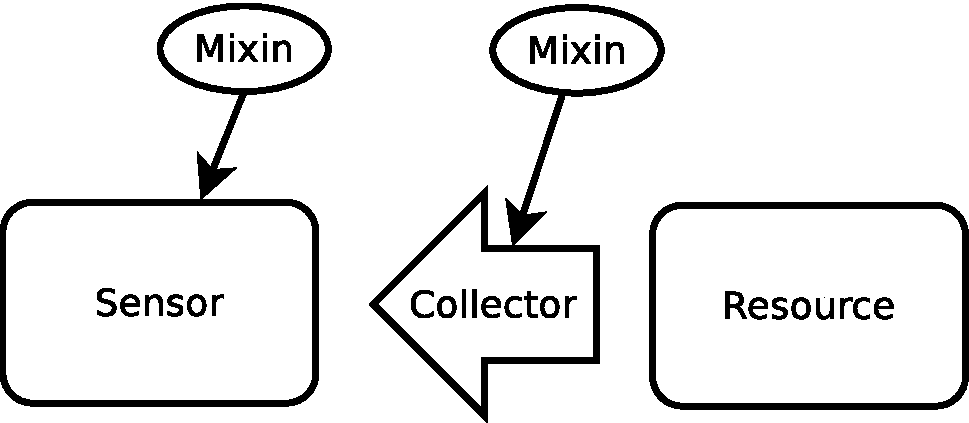
\includegraphics[width=0.5 \linewidth]{onestage.pdf}
\caption{The simplest case: one \coll\ and one \sens\ \label{fig:onestage}}
\end{figure}

Although the interface based on \sens s and \coll s may describe very simple use cases with minimal effort, the designer is able to assemble complex, multilayer monitoring infrastructures using the same basic building blocks: for instance, a \sens\ can be used to aggregate a storage throughput using the input from three \coll s, one for the average response time, one for the mean time between failures, and another for network delay, and provide the results to an upstream \sens\ that aggregates the same results from other \sens s.

%The {\em Resource Management} box stands for a resource that is the end-user of the monitoring activity. It's {\em Kind} is bound to the publishing technique used in the \coll . It may be, for instance, a {\em Compute} resource that embeds a load balancing or accounting functionality, or a yet to define {\em Mailbox} resource where periodic reports are posted. 

\rem{author}{Why not a mixin to the monitored resource directly? I envision problems emerging with the implementation. A resource can be ``prepared'' for monitoring, but the way in which the Monitoring Link will interact with such preparation is not clear. In addition, consider that the same tool might be the target of several links, with distinct configuration parameter. How can the control parameters of the mixin be exposed in such a case? Instead, if the mixin is embedded in the link, it is the responsibility of the link implementation to configure it, and to couple it with the publishing technology indicated in the link}

We point out that the interface is transparent to the existence of a standard for metric identifiers: if one exists, the interoperability of distinct monitoring infrastructures is certainly improved. We consider that the user that interacts with the monitoring infrastructures either knows about the identifiers used by the provider, or uses an interface (e.g., a SLA negotiation service) that translates provider specific identifiers into interoperable ones. This document highlights other similar standardization issues.

Summarizing, the specifications introduced in this document require that the conformant provider implements two {\em Kind}s: the {\em \coll } and the {\em \sens }. Three generic \mi s are also defined to enable the classification of \mi s that are specific for the provider: namely {\em ToolSet} to specify the production of measurement, {\em AggregatorSet} for their processing, and {\em PublisherSet} for their publication. The generic \mi s are used to identify and apply restrictions to provider-specific \mi s. 

\subsection{Terminology shortcuts}

To distinguish a {\em Resource} instance from its {\em Kind}, we will use the indeterminative article for the instance (e.g., ``a \rs''), and the determinative article for the {\em Kind} (e.g., ``the \rs''). The plural is reserved to instances (e.g., ``the \rs s''). In case of ambiguity we will further specify ``instance'' or ``{\em Kind}''. 

Similarly, we will use the term {\em a $<$mixin id$>$ \mi} to indicate a \mi\ that {\em depends} on the {\em $<$mixin id$>$} \mi. The provider ensures that \mi s inherit defined semantics from the \mi\ they depend on, as explained in the rest of this paper. 

\section{Specification of the compliant server}

The compliant server MUST define the following {\em Kind}s:

\begin{description}

\item [\coll] that describes how monitoring results are collected and trasferred between {\em Resource}s (see table \ref{tab:collector});

\item [\sens] that describes how monitoring results are aggregated (see table  \ref{tab:sensor});

\end{description}

In addition, the compliant server MUST define the following {\em Mixin}s (see table \ref{tab:mixin}): 

\begin{description}

\item [{\em ToolSet}] that is used to apply restrictions on the \mi s describingMonitoring tools associated with a \coll;

\item [{\em AggregatorSet}] that is used to apply restrictions on the \mi s describing the aggregation function operated by a \sens;

\item [{\em PublisherSet}] that is used to apply restrictions on the \mi s that describe the technique used by the \sens\ to publish monitoring results;

\end{description}

\begin{table}
\scriptsize
\mixin{AggregatorSet}{None}

\mixin{ToolSet}{None}

\mixin{CollectorSet}{None}

\caption{Definition of the \mi s collections \label{tab:mixin}}
\end {table}


\subsection{The \coll}

\begin{table}
\scriptsize
\link{\coll}{(see below)}

\attributes{Collector Link}{
occi.collector.period & number & true & true & The time between two following measurements \\
occi.collector.periodspec & string & true & false & granularity, accuracy, exponent of period measument \\
}
\caption{Definition of the \coll\ Kind \label{tab:collector}}
\end {table}


The \coll\ models  (see table \ref{tab:collector}) the transfer of metric measurements from one \rs\ to a \sens . The {\em target} attribute of a \coll\ MUST correspond to a \sens .

A \coll\ is characterized by the activity that extracts metric measurements from the source \rs.

Only the timing of the monitoring activity is defined by OCCI attributes defined for the \coll\ {\em kind}, similar to those defined for the \sens . Other attributes of the \coll\ are defined by {\em ToolSet} \mi s. 

\subsection{The \sens \label{sec:sensor}}

\begin{table}
\scriptsize
\resource{\sens}{(see below)}

\attributes{Sensor Resource}{
occi.sensor.period & number & true & true & The time between two following measurements \\
occi.sensor.periodspec & string & true & false & granularity, accuracy, exponent of period measument \\
occi.sensor.timebase & number & false & true & The server time when the timestart and timestop are modified \\  
occi.sensor.timestart &	number & true & true & The delay after which the session is planned to start \\
occi.sensor.timestop & number	& true & true & The delay after which the session is planned to stop \\
occi.sensor.timespec & string & true & false & granularity, accuracy, exponent of time measurement \\
}
\caption{Definition of the {\em Sensor Resource} Kind \label{tab:sensor}}
\end {table}


The \sens\ (see table \ref{tab:sensor}) models the processing of the measurements, like their aggregation in composite metrics, as well as their publishing.

A \sens\ is characterized by OCCI attributes that define the rate with which new observations are produced, and by the scheduling times of its operation. The attributes with \verb|required=true| MUST be assigned a legal value upon instantiation. The server MUST reject an incomplete instantiation.

The execution rate is defined using three attributes: the rate itself, and an optional definition of the quality of the timing. This latter attribute contains a triple of numbers encoded as a string, that define the granularity with which the rate is measured, and the accuracy of rate measurement, and the floating point exponent. By default \verb|periodspec="NaN, NaN, 0"|.

The activation of a \sens\ is controlled by two attributes that describe the scheduling of sensor activity: to schedule the execution of a sensor the user modifies the {\tt starttime} with a value indicating how far in the future the instance is going to start its activity. A value of zero corresponds to the immediate start. The server sets the {\tt timebase} attribute corresponding to the reference time of the start time.

All time values are represented as numbers. The {\tt timebase} corresponds to Unix seconds, all timing values use a floating point notation. Also for time values there is a {\tt timespec} attribute analogous to {\tt periodspec}.

To define its operation, a \sens\ is associated with \mi s that depend on {\em AggregatorSet} and {\em PublisherSet} \mi s.


\subsection{Restrictions on \mi s that depend on {\em ToolSet} \label{sec:Tool}}

The measurement activity is integrated in the \coll\ using a {\em ToolSet} \mi . Such a \mi\ implements a measurement activity on the \rs that is the source of the \sens\ the \mi\ is associated with.

In principle, each provider may associate a different semantic to a given \mi, so here there is ground for further standardization. If the provider does not adhere to a defined standard, it MUST give an exhaustive documentation of the monitoring tool associated with a \mi.

To enable interoperabilty, the provider SHOULD follow a defined standard for the naming of input, control and result attributes, but its specification falls outside the scope of this document. Such naming MAY help the discovery of \mi\ that are appropriate for a given task.

The attributes are divided into two groups:
\begin{itemize}
\item Control attributes: they control the operation of the measurement activity. For instance a \mi\ implementing a ping tool may have a control attribute defined as 
\begin{verbatim}
name=size,type=string,mutable="true",required="false",default=84
\end{verbatim}
The role of the attributes is part of the specification of the specific \mi.
\item Metric attributes: they correspond to the metrics delivered to the target \sens, and SHOULD hold a reasonably updated value for those metrics. In principle, each provider may associate a different semantic to a given \mi, so here there is ground for further standardization. If the provider does not adhere to a defined standard, it MUST give an exhaustive documentation of the monitoring tool associated with a \mi.
\end{itemize}

To enable interoperabilty, the provider SHOULD follow a defined standard for the naming of metric and control attributes, but its specification falls outside the scope of this document. Such naming MAY help the discovery of \mi\ that are appropriate for a given task.

The metric attributes of the {\em ToolSet} \mi\ associated a \coll\ instance contribute to the scope of the target \sens\ referenced in sect. \ref{sec:Aggregator}.

\subsection{Restrictions on \mi s that depend on {\em AggregatorSet} \label{sec:Aggregator}}

A \mi\ that depends on the {\em AggregatorSet} \mi\ is meant to implement the computation of an aggregated metric starting from raw metrics: it represents the function applied by a \sens. In principle, each provider has a distinct offer of such \mi s, so here there is ground for further standardization. If the provider does not adhere to a defined standard, it MUST give an exhaustive documentation of the aggregation functions associated with a \mi.

The attributes of a \mi\ that depends on the {\em AggregatorSet} are divided into three groups:

\begin{itemize}
\item Input attributes: they bind a metric in the scope of the \sens\ with an input of the aggregating function. The scope of a \sens\ consists of the {\tt name}s of all the metric attributes of the incoming \coll s and of the {\em AggregatorSet} \mi s associated with the same \sens . A metric indicated as the value of an input attribute MUST be in the scope of the \sens . For instance, a \sens\ that implements a EWMA may have an {\tt input} attribute equal to 
\begin{verbatim}
data="com.provider.monitoring.collector1.roundtrip"
\end{verbatim}
where \verb&roundtrip& is a metric delivered by an incoming \coll\ {\tt collector1}.
\item Control attributes: they control the operation of the aggregating function (for instance, the gain of an EWMA);
\item Metric attributes: they correspond to the metrics delivered. Their value SHOULD correspond to the last computed value. They also contribute to the scope of the \sens\ they are associated with.
\end{itemize}

To enable interoperabilty, the provider SHOULD follow a defined standard for the naming of input, control and result attributes, but its specification falls outside the scope of this document. Such naming MAY help the discovery of \mi\ that are appropriate for a given task.

\subsection{Restrictions on \mi s that depend on {\em PublisherSet} \label{sec:Publisher}}

How data are delivered is defined by a {\em PublisherSet} \mi .

In principle, each provider may associate a different semantic to similar \mi s, so here there is ground for further standardization. If the provider does not adhere to a defined standard, it MUST give an exhaustive documentation of the publishing mode associated with this \mi.

Examples of measurement delivery modes are through a Unix pipe, on demand through a TCP connection, pushed using UDP datagrams, persistently recorded in a database.

The attributes of a {\em PublisherSet} \mi\ are divided into two groups:

\begin{itemize}
\item Input attributes: their value MUST correspond to URIs of one of the metrics in the scope of the \sens.
\item Control attributes: they determine the process used to publish input attributes.
\end{itemize}

To enable interoperabilty, the provider SHOULD follow a defined standard for the naming of input and control attributes, but its specification falls outside the scope of this document. Such naming MAY help the discovery of \mi s that are appropriate for a given task.

\subsection{Constraints on the associations between instances and \mi s}

The constraints on the association of \sens\ and \coll\ instances with the defined \mi s are the following:

\begin{itemize}

\item a {\em Sensor Resource} MUST be the {\em target} of at least one \coll ;

\item the {\em target} of a {\em \coll} MUST be a \sens ;

\item a {\em ToolSet} \mi\ can be associated ONLY with a \coll;

\item an {\em AggregatorSet} \mi\ can be associated ONLY with a \sens;

\item a {\em PublisherSet} \mi\ can be associated ONLY with a \sens.

\end{itemize}

\rem{author}{The utilization of \mi s, instead of kind-specific attributes describing the operation, has the purpose of allowing the discovery of the capabilities offered by the provider. Kind specific attr. might be three, describing the tool id, and ohter two formatted strings for the input and output parameters}

\section{Conformance profiles}

The definition of conformance profiles is appropriate because the provision of an interface for the management of a monitoring infrastructure is optional. 

\begin{description}

\item[Profile 0] The \coll\ and \sens\ {\em Kind} s MUST NOT be implemented: attempt of instantiating such {\em Kinds} fails.  In an HTTP rendering a POST and GET over the corresponding URI returns {\tt 404 Notfound}. The {\em AggregatorSet}, {\em ToolSet}, and {\em PublisherSet} \mi s MUST NOT be implemented: discovery fails. In an HTTP rendering a GET over the \mi\ returns {\tt 404 Notfound}; 

\item[Profile 1] The \coll\ and \sens\ {\em Kind} s MUST be implemented, and the user MUST be allowed to create new instances of such {\em Kinds}.  In an HTTP rendering a POST or a GET over the corresponding URI return respectively {\tt 201} and {\tt 200}. In case of error, the server MUST NOT return {\tt 404 Notfound}. The {\em AggregatorSet}, {\em ToolSet}, and {\em PublisherSet} \mi\ MUST be implemented, and discovery is successful. The server MUST NOT allow to introduce {\em depends} relationships with the {\em AggregatorSet}, {\em ToolSet}, and {\em PublisherSet} \mi s. In an HTTP rendering, a POST over their URIs returns {\tt 405 Method Not allowed}; 

\item[Profile 2]  The \coll\ and \sens\ {\em Kind} s MUST be implemented, and the user MUST be allowed to create new instances of such {\em Kinds}.  In an HTTP rendering a POST and GET over the corresponding URI returns respectively {\tt 201} and {\tt 200}. In case of error, the server MUST NOT return {\tt 404 Notfound}. The {\em AggregatorSet}, {\em ToolSet}, and {\em PublisherSet} \mi s MUST be implemented, and discovery is successful. The user MUST be allowed to introduce {\em depends} relationships with the  {\em AggregatorSet}, {\em ToolSet}, and {\em PublisherSet} \mi s. In an HTTP rendering, a POST over their URIs returns {\tt 200}.

\end{description}

\section{Related works}

The model is reminiscent of a monitoring infrastructure that I designed and implemented in the CoreGRID EU-project \cite{cur:08:a}, that in its turn is inspired by various other works (see the bibliography in the paper). The reading of the CompatibleOne prototype \cite{mar12a} has been enlightening concerning (among the rest) the need and possibility of modularizing the monitoring part. The 2012 revision of the OCCI core model \cite{occi:core} has been used as a reference.


\section{Security Considerations}
\label{s:security}

The API described in this document relies on the same mechanism as the basic OCCI API, of which it is an extension. In its turn, the OCCI API is designed according with a RESTFul model, a style of exposing a web service to the users.

The way this API is exposed inherits the security aspects of the RESTFul model, that can be summarized as follows:

\begin{itemize}
\item the web site MUST be protected to allow access only to authorized users, and to protect the content of the communication;
\item the content uploaded on the web site by the user (using POST) MUST be protected;
\item the content cached on third party sites not directly accessible by the user and by the provider (proxies etc.) MUST be protected.
\end{itemize}

We stress that these security warnings are shared with any ReStFul API.

The provider must ensure that a user defined \mi\ does not compromise the security of other services. The provider may attain this by restricting the functionalities associated to a \mi\ (the limit case is the provision of templates) or run the functionalities associated to a \mi\ in a protected environment (e.g., as a Unix user in a chroot jail). This issue is shared with the OCCI model.

Concerning the kind of monitoring infrastructure deployed using the \sens\ and the \coll , security aspects are managed using appropriate \mi s. For instance the \coll\ might be associated with a \mi\ describing a secure transport protocol, while the sensor might be configured to be accessible only from authenticated users (?). The provider SHOULD offer the user a set of predefined \mi s that introduce the appropriate level of security. User defined \mi s SHOULD be avoided for this kind of options.



\todo{update glossary}

\begin{tabular}{l|p{12cm}}
Term & Description \\
\hline
\hl{Action} & An OCCI base type. Represents an invocable operation on a \hl{Entity} sub-type instance or collection thereof. \\

\hl{Attribute} & A type in the OCCI Core Model. Describes the name and properties of attributes found in \hl{Entity} types. \\

\hl{Category} & A type in the OCCI Core Model and the basis of the OCCI type identification mechanism. The parent type of \hl{Kind}. \\

capabilities & In the context of \hl{Entity} sub-types {\bf  capabilities} refer
  to the OCCI \hl{Attribute}s and OCCI \hl{Action}s exposed by an {\bf entity
  instance}. \\

\hl{Client} & An OCCI client.\\

\hl{Collection} & A set of \hl{Entity} sub-type instances all associated to a particular \hl{Kind} or \hl{Mixin} instance. \\

\hl{Entity} & An OCCI base type. The parent type of \hl{Resource} and \hl{Link}. \\

entity instance & An instance of a sub-type of \hl{Entity} but not an instance
  of the \hl{Entity} type itself.  The OCCI model defines two sub-types of
  \hl{Entity}, the \hl{Resource} type and the \hl{Link} type.  However, the
  term {\em entity instance} is defined to include any instance of a
  sub-type of \hl{Resource} or \hl{Link} as well. \\

\hl{Kind} & A type in the OCCI Core Model. A core component of the OCCI classification system. \\

\hl{Link} & An OCCI base type. A \hl{Link} instance associates one \hl{Resource} instance with another. \\

\hl{Mixin} & A type in the OCCI Core Model. A core component of the OCCI classification system. \\

mix-in & An instance of the \hl{Mixin} type associated with an {\em entity
 instance}. The ``mix-in'' concept as used by OCCI {\em only} applies to
 instances, never to \hl{Entity} types. \\

model attribute & An internal attribute of a the Core Model which is {\em not}
  client discoverable. \\

\hl{OCCI} & Open Cloud Computing Interface. \\

OCCI base type & One of \hl{Entity}, \hl{Resource}, \hl{Link} or \hl{Action}. \\

OCCI Action & see \hl{Action}. \\
OCCI Attribute & A client discoverable attribute identified by an instance of the \hl{Attribute} type. Examples are \hl{occi.core.title} and \hl{occi.core.summary}. \\
OCCI Category & see \hl{Category}. \\
OCCI Entity & see \hl{Entity}. \\
OCCI Kind & see \hl{Kind}. \\
OCCI Link & see \hl{Link}. \\
OCCI Mixin & see \hl{Mixin}. \\

OGF & Open Grid Forum. \\

\hl{Resource} & An OCCI base type. The parent type for all domain-specific \hl{Resource} sub-types. \\

resource instance & See {\em entity instance}. This term is considered obsolete. \\

tag & A \hl{Mixin} instance with no attributes or actions defined. \\

template & A \hl{Mixin} instance which if associated at instance
creation-time pre-populate certain attributes. \\

type & One of the types defined by the OCCI Core Model.  The Core Model types are
 \hl{Category}, \hl{Attribute},
 \hl{Kind}, \hl{Mixin}, \hl{Action}, \hl{Entity}, \hl{Resource}
 and \hl{Link}. \\

concrete type/sub-type & A concrete type/sub-type is a type that can be instantiated.\\

URI & Uniform Resource Identifier. \\
URL & Uniform Resource Locator. \\
URN & Uniform Resource Name. \\
\end{tabular}


\section{Contributors}

\textbf{Augusto Ciuffoletti (corresponding author)} \\
Dept. of Computer Science \\
L.go B. Pontecorvo - Pisa\\
Italy \\
Email: augusto.ciuffoletti@gmail.com \\

\textbf{Andrew Edmonds}\\
Institute of Information Technology \\
Zürich University of Applied Sciences \\
Zürich \\
Switzerland \\
Email: andrew.edmonds@zhaw.ch

\textbf{Metsch, Thijs} \\
Intel Ireland Limited \\
Collinstown Industrial Park \\
Leixlip, County Kildare, Ireland
Email: thijsx.metsch@intel.com

\textbf{Ralf Nyren} \\
Email: ralf@nyren.net 

%\section{Acknowledgments}

%Include if desired. Contributors to the document may also be listed in the previous section.

\appendix

\section*{Appendix - An example}

We want to dip the Monitoring Infrastructure Management schema explained in this document into an Service Level Agreement (SLA) scenario, so let's try to define a SLA in terms of OCCI concepts.

An OCCI-SLA is a contract between a user and a provider: the terms of the contract are in a form that may be provider-independent, and they are published as an OCCI-Resource in a specific namespace "occi/\#sla" possibly refined with mixins. There are two basic flavors for a SLA contract:

\begin{itemize} 
\item The provider offers a SLA: the providers offers the user the ability to monitor the conformance to SLA contract
\item The user offers a SLA: the provider offers the User the tools to implement resource monitoring to meet internal SLA requirements.
\end{itemize}

Both of them are compatible with the monitoring infrastructure management schema illustrated in this paper, but are otherwise quite different.

The Service Level Agreement is an aggregate of many \rs\, that describe financial, administrative, security aspects and much more. Among such \rs\, there are the Service  Objectives (SLO). Their function is to specify the meaning of "quality of service" for the specific infrastructure. This concept is translated in a function of system parameters of operation, or metrics.
 The SLA resource contains the instructions to associate an action to a given SLO pattern.

A user that wants to instantiate a monitoring infrastructure starts from identifying the Resources and the metrics of interest. Next the basic monitoring infrastructure is instantiated, assembling generic \sens s and \coll s. The following step consists of browsing {\em ToolSet} \mi s finding one that offers the right metrics, and the first stage \coll\ is associated with it. Note that a given monitoring technology may require more than one \coll\ to operate (e.g., consider iperf). Another {\em AggregatorSet} \mi\ for the \sens\ is discovered, and the \sens\ is associated with it. Finally, a publishing technology is selected from the \mi\ that depend on {\em PublisherSet} \mi , and the \sens\ is associated with it.

The following example gives a more detailed insight of the process: it illustrates a \sens\ that measures processor utilization for a given virtual machine {\tt vm1}, and triggers an alarm when the idle time becomes less than 10\%. The alarm message is pushed as a UDP packet injected in a VLAN. We refer to the HTTP rendering to give a better insight of the operation. The object diagram is in figure \ref  {fig:example}

\begin{figure}
\centering
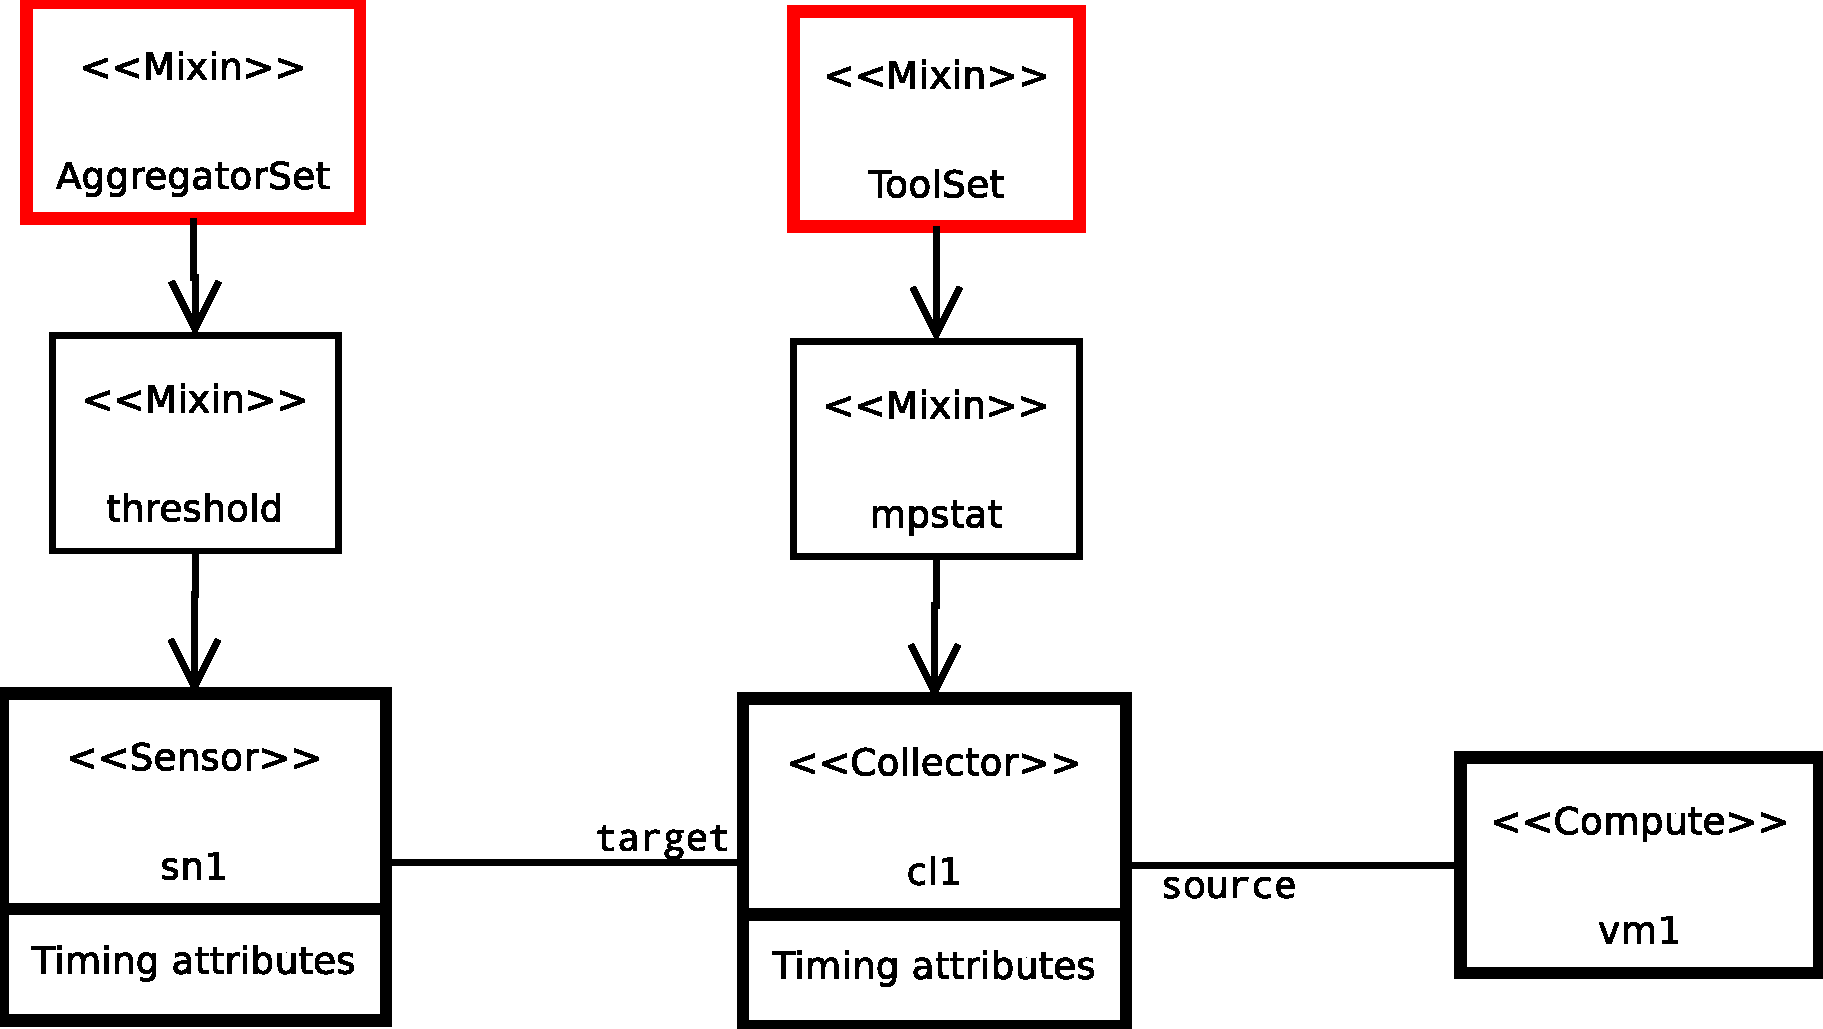
\includegraphics[width=0.7 \linewidth]{Diagram.pdf}
\caption{The instance diagram of the monitoring infrastructure \label{fig:example}}
\end{figure}

The user starts instantiating a new \sens, and a \coll\ connecting {\tt vm1} to the sensor. The new \sens:

\begin{verbatim}
> POST /sensor/ HTTP/1.1
> Category: sensor; 
            scheme:"http://schemas.ogf.org/occi/monitoring#"; 
            class="kind"
...
< HTTP/1.1 201 OK
< Location: "http://provider.com/monitoring/sn1
\end{verbatim}

the input \coll:

\begin{verbatim}
> POST /collector/ HTTP/1.1
> Category: collector;
>           scheme="http://schemas.ogf.org/occi/monitoring#";
>           class="kind";
> X-OCCI-Attribute: occi.core.target="http://provider.com/monitoring/sn1
> X-OCCI-Attribute: occi.core.source="http://provider.com/vms/vm1
> ...
...
< HTTP/1.1 201 OK
< Location: "http://provider.com/monitoring/cl1
\end{verbatim}

The timing attributes of the two instances are filled in

\begin{verbatim}
> POST /monitoring/sn1/ HTTP/1.1
> ...
> X-OCCI-Attribute: occi.sensor.period=10;
> X-OCCI-Attribute: occi.sensor.periodspec="1,0.1,1";
> X-OCCI-Attribute: occi.sensor.timestart=10
> X-OCCI-Attribute: occi.sensor.timestop=3600;
> X-OCCI-Attribute: occi.sensor.timegranularity="1,0.1,1";
\end{verbatim}

\begin{verbatim}
> POST /monitoring/cl1/ HTTP/1.1
> ...
> X-OCCI-Attribute: occi.collector.period=10;
> X-OCCI-Attribute: occi.collector.periodspec="1,0.1,1";
\end{verbatim}

The monitoring activity will start in 10 seconds and last for 1 hour, performing one measurement every 10 seconds. Granularity and accuracy are just consistent with the timing requirements.

Next, the user browses the \mi s that depend on the {\tt ToolSet} \mi\ looking for a tool that measures processor idle time: the search pattern comes from outside our scenario. We may envision a query like the following:

\begin{verbatim}
> GET /-/toolset/ HTTP/1.1
> ...
attribute=idletimecpu
\end{verbatim}

where the user indicates the metric of interest (idletimecpu) as one of the attributes. The provider may return one or more \mi s, and we consider that one of them is {\tt mpstat}, as defined in table \ref{tab:mpstat} in the provider's namespace {\tt http://provider.com/monitoring/}.

\begin{table}
\scriptsize
\extramixin{mpstat}{(see table below)}{toolset}

\attributes{mpstat \mi}{
com.provider.mpstat.port & number & true & true &  The port where to send a measurement trigger (control) \\
com.provider.mpstat.ncpu & number & false & true & The number of processors (metric) \\ 
com.provider.mpstat.idletimecpu & number & false & true & Total percent of idle time (metric)  \\ 
com.provider.mpstat.usertimecpu & number & false & true & Total percent of user time (metric) \\
com.provider.mpstat.systimecpu & number & false & true & Total percent of system time (metric) \\
}
\caption{Attributes defined for the {\tt mpstat} mixin \label{tab:mpstat}}
\end {table}

Then it associates {\tt cl1} with the {\tt mpstat} \mi:

\begin{verbatim}
> POST /toolset/mpstat/ HTTP/1.1
> X-OCCI-Location: http://provider.com/monitoring/cl1
\end{verbatim}

This latter operation is critical, and may give rise to a number of errors, that result in 4xx and 5xx error codes. For instance, the server may return {\tt 403 Forbidden} in the case the {\tt ToolSet} \mi\ is not legal for the target resource.

In the general case, the above steps are repeated for every metric that the user needs to measure to compute the application-dependent metric. Here we proceed to the next step. 

The user now searches in a similar way an {\tt AggregatorSet} \mi\ that returns a threshold signal: it finds the {\tt Threshold} defined in table \ref{tab:vat}

\begin{table}
\scriptsize
\extramixin{threshold}{(see table below)}{aggregatorset}

\attributes{threshold}{
com.provider.threshold.threshold & number & true & true & The threshold value (control) \\
com.provider.threshold.mode & {Once,Continuous} & true & true & How frequent the warning message (control) \\ 
com.provider.threshold.fallmsg & String & true & true & The falling edge message (control)\\
com.provider.threshold.risemsg & String & true & true & The rising edge message (control)\\
com.provider.threshold.input & URI & false & true & The input value (input)  \\  
com.provider.threshold.message & String & false & true & The output string (metric)  \\  
}
\caption{Attributes defined for the {\tt threshold} mixin \label{tab:vat}}
\end {table}

The next step of the user is to associate the \sens\ to the \mi,

\begin{verbatim}
> POST /computetool/threshold/ HTTP/1.1
> ...
> X-OCCI-Location: http://provider.com/monitoring/sn1
\end{verbatim}
 
and fills in the attributes as appropriate:

\begin{verbatim}
POST /monitoring/sn1/ HTTP/1.1
> ...
> X-OCCI-Attribute: com.provider.threshold.threshold=10
> X-OCCI-Attribute: com.provider.threshold.mode="Once"
> X-OCCI-Attribute: com.provider.threshold.fallmgs="Warning: vm1 overloaded"
> X-OCCI-Attribute: com.provider.threshold.risemgs="vm1 load below 90%"
> X-OCCI-Attribute: com.provider.threshold.input="com.provider.monitoring.tool1.idletimecpu"
\end{verbatim}

The server here responds with a {\tt 404 Not found} if the {\tt input} attribute does not exist, or {\tt 401 Unauthorized} if the user is not allowed to operate on that \rs\ (e.g., the metric is outside its scope).

Finally the user associates a way to publish the result: a UDP datagram on a network. It looks or a {\tt PublisherSet} \mi\ that applies, and finds the one described in figure \ref{tab:udp}, that sends a string as a UDP datagram.

\begin{table}
\scriptsize
\extramixin{udptxtdgm}{(see table below)}{collectorset}

\attributes{udptxtdgm}{
com.provider.udptxtdgm.UDPdest & String & true & true & The destination of the message (control) \\
com.provider.udptxtdgm.UDPport & number & true & true & The destination port (control) \\ 
com.provider.udptxtdgm.mode & {all,nonempty} & true & true & Indicate whether only non empty msg are sent (control) \\ 
com.provider.udptxtdgm.input & URI & true & true & The msg to be sent \\
}
\caption{Attributes defined for the {\tt udptxtdgm} mixin \label{tab:udp}}
\end {table}

It then associates that \mi\ to the outgoing \coll:

\begin{verbatim}
> POST /collectorset/udptxtdgm/ HTTP/1.1
> ...
> X-OCCI-Location: http://provider.com/monitoring/collector2
\end{verbatim}

and fills in the attributes as appropriate:

\begin{verbatim}
POST /monitoring/sn1/ HTTP/1.1
> ...
> X-OCCI-Attribute: com.provider.udptxtdgm.UDPdest="ctr1.provider.com";
> X-OCCI-Attribute: com.provider.udptxtdgm.UDPport="10222";
> X-OCCI-Attribute: com.provider.udptxtdgm.mode="nonempty";
> X-OCCI-Attribute: com.provider.udptxtdgm.input="http://provider.com/monitoring/sn1/message";
\end{verbatim}


\section{Intellectual Property Statement}

The OGF takes no position regarding the validity or scope of any intellectual property or other rights that might be claimed to pertain to the implementation or use of the technology described in this document or the extent to which any license under such rights might or might not be available; neither does it represent that it has made any effort to identify any such rights.  Copies of claims of rights made available for publication and any assurances of licenses to be made available, or the result of an attempt made to obtain a general license or permission for the use of such proprietary rights by implementers or users of this specification can be obtained from the OGF Secretariat.

The OGF invites any interested party to bring to its attention any copyrights, patents or patent applications, or other proprietary rights which may cover technology that may be required to practice this recommendation.  Please address the information to the OGF Executive Director.

\section{Disclaimer}

This document and the information contained herein is provided on an ``As Is'' basis and the OGF disclaims all warranties, express or implied, including but not limited to any warranty that the use of the information herein will not infringe any rights or any implied warranties of merchantability or fitness for a particular purpose.

\section{Full Copyright Notice}

Copyright \copyright \ Open Grid Forum (\copyrightyears). Some Rights Reserved.

This document and translations of it may be copied and furnished to others, and derivative works that comment on or otherwise explain it or assist in its implementation may be prepared, copied, published and distributed, in whole or in part, without restriction of any kind, provided that the above copyright notice and this paragraph are included as references to the derived portions on all such copies and derivative works. The published OGF document from which such works are derived, however, may not be modified in any way, such as by removing the copyright notice or references to the OGF or other organizations, except as needed for the purpose of developing new or updated OGF documents in conformance with the procedures defined in the OGF Document Process, or as required to translate it into languages other than English. OGF, with the approval of its board, may remove this restriction for inclusion of OGF document content for the purpose of producing standards in cooperation with other international standards bodies. 

The limited permissions granted above are perpetual and will not be revoked by the OGF or its successors or assignees. 



% \phantomsection\addcontentsline{toc}{section}{References}
\section{References}

% Define heading of bibliography to be empty, since we already have a heading above the text.
\renewcommand{\refname}{}
\vspace*{-3em}

% Use bibliography.bib for references.
\bibliography{biblio,cur}

% Alternatively, you can insert the bibliography inline, like so:
% 
% \begin{thebibliography}{5}
% 
% \bibitem[GFD0000()]{gfd0000}
% Firstname Author1 and Firstname Author2.
% \newblock {Our Awesome Grid Forum Document}.
% \newblock GWD-C.0000, April 2002.
% 
% \bibitem[GFD152()Catlett, de~Laat, Martin, Newby, and Skow]{gfd152}
% Charlie Catlett, Cees de~Laat, David Martin, Gregory~B. Newby, and Dane Skow.
% \newblock {Open Grid Forum Document Process and Requirements}.
% \newblock GFD-C.152, June 2009.
% \newblock URL \url{http://www.ogf.org/documents/GFD.152.pdf}.
% 
% \bibitem[RFC2119()]{rfc2119}
% Scott Bradner.
% \newblock {Key words for use in RFCs to Indicate Requirement Levels}.
% \newblock RFC 2119 (Best Current Practice), March 1997.
% \newblock URL \url{http://tools.ietf.org/html/rfc2119}.
% 
% \bibitem[RFC3552()Rescorla, Korver, and {Internet Architectures Board}]{rfc3552}
% Eric Rescorla, Brian Korver, and {Internet Architectures Board}.
% \newblock {Guidelines for Writing RFC Text on Security Considerations}.
% \newblock RFC 3552 (Best Current Practice), July 2003.
% \newblock URL \url{http://tools.ietf.org/html/rfc3552}.
% 
% \bibitem[RFC3967()]{rfc3967}
% Randy Bush and Thomas Narten.
% \newblock {Clarifying when Standards Track Documents may Refer Normatively to Documents at a Lower Level}.
% \newblock RFC 3967 (Best Current Practice), December 2004.
% \newblock URL \url{http://tools.ietf.org/html/rfc3967}.
% 
% \end{thebibliography}



\end{document}
